\newcommand{\TODO}{\hl{\emph{TODO:}}\hl}
%Get rid of the above when done.

\chapter{Simulating Virtual Creatures}

\section{Karl Sims}

In 1994, a researcher named Karl Sims simulated Darwinian evolution by breeding 
virtual block creatures to accomplish tasks such as running, jumping, and following 
light sources in a physical environment. His work was groundbreaking in that he didn't 
start by designing a control algorithm or a body for his creatures; the creatures 
evolved complex brains and bodies {\em without human intervention}. Sims used 
{\em genetic algorithms}, which can be used to approach problems with large solution 
spaces that are computationally expensive to define.
\index{Sims, Karl}
\index{Evolution, Darwinian}

\begin{ex}
  Watch some of Karl Sims' creatures on YouTube:
  \url{youtube.com/watch?v=JBgG_VSP7f8}. Do they remind you of real world
  animals? Since the creatures he started with were randomly generated, how can that be?
\end{ex}

\begin{ex}
  Read the paper that Karl Sims presented at Siggraph:
  \url{karlsims.com/papers/siggraph94.pdf}. How does he think his
  work will be useful in the future?
\end{ex}

\section{Genetic Algorithms}

Genetic algorithms (GAs) are based on our understanding of the process of 
natural evolution. In a nutshell, the {\em fittest} of a population of possible 
solutions survive to form a new (hopefully better) population, and the process
repeats itself until an end condition is reached (for example, when an optimal
solution has been found). 
\index{Genetic Algorithms}

\begin{enumerate}
  \item Generate an initial population of {\em genotypes} that encode potential
  {\em phenotypes} (solutions). This initial population is usually random.

  \item Evaluate the ``goodness'' of each phenotype in the population using a 
  {\em fitness} function. \label{GA:GoodnessStep}

  \item Select $n$ phenotypes probabalistically such that fit phenotypes 
  are more likely to be selected.

  \item Breed the genotypes corresponding to the selected phenotypes by combining 
  traits of the existing genotypes and {\em mutating} some of them randomly. 
  The specfics of the breeding process depend heavily on the implementation of the algorithm.
  The result of this step is a new population of genotypes that will be used in
  the next generation of the algorithm.\footnote{This population is usually the
  same size as the original population.} 

  \item Repeat steps \ref{GA:GoodnessStep}-\ref{GA:LoopStep} with each new generation 
  until an optimal solution has been identified, the algorithm has run for the maximum 
  number of generations, or some other terminal condition is triggered. \label{GA:LoopStep}

\end{enumerate}
\index{genotype}
\index{phenotype}

Genetic algorithms are a subset of {\em Evolutionary Algorithms}, which you can
read about at \url{wikipedia.org/wiki/Evolutionary_algorithm}.

How do genetic algorithms solve problems? All possible solutions to a problem
exist within a {\em solution space} and a genetic algorithm is a type of
{\em search algorithm} for finding the optimal solution in that space.

\beforefig
\centerline{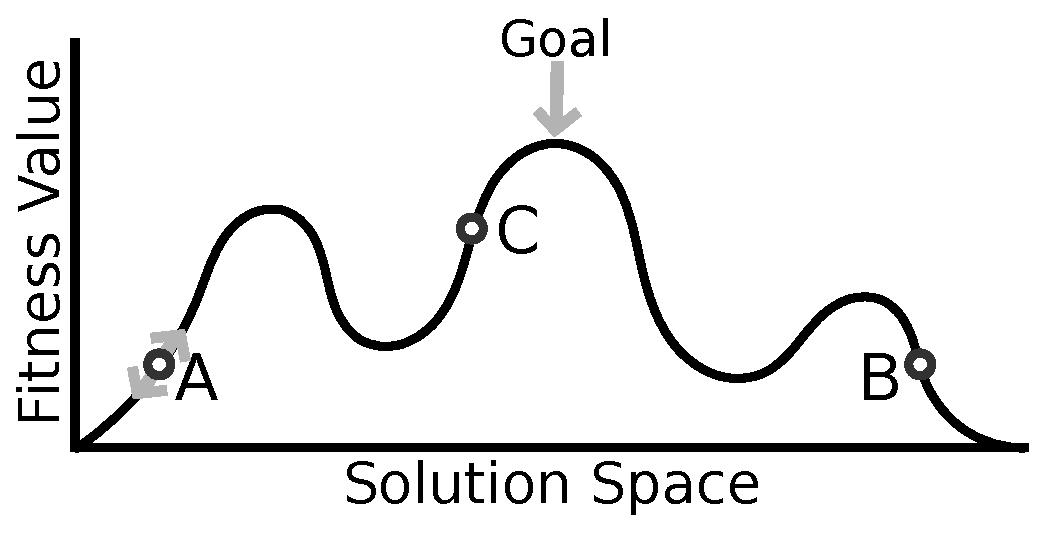
\includegraphics[width=2in]{./pycritters_figs/GeneticAlgStateSpace.eps}}
\afterfig

In the diagram above, {\tt A} and {\tt B} represent randomly generated
individuals with relatively low fitness values. During breeding, there is a
chance that a trait is mutated. This usually results in a lower fitness value,
but can at times be beneficial, as the arrows around {\tt A}
indicate.\footnote{Depending on the trait being mutated and the degree of
mutation, it is also possible that the resulting solution could lie on a
different hill in the solution space.} Breeding between two individuals
generally involves a {\em crossover} of traits between those individuals, 
with the goal of mixing good behaviors in order to create a new individual 
on a different hill in the solution space. For example, breeding {\tt A} 
and {\tt B} could result in {\tt C} in the diagram above, which is closer 
to the global maximum than either of its parents.
 
\begin{ex}
  Read more about genetic algorithms on wikipedia: 
  \url{http://en.wikipedia.org/wiki/Genetic_algorithm}. List several ways that 
  genotypes in a population could be represented.
\end{ex}

% Could be too much of a leap
\begin{ex}
  Read about the 8 queens problem at \url{wikipedia.org/wiki/8_queens}.
  Try to solve it using a genetic algorithm. Hint: you can represent
  each possible solution as a string where each character is a number
  between 0 and 7.
\end{ex}

\section{A Simple Brain Model}

Karl Sims' creatures were driven by control systems called {\em artificial neural
networks}, directed small world graphs that model the behavior of biological brains and
have been used successfully to perform non-linear data analysis in fields such as
pattern matching and image recognition.
\index{neural networks}

The basic unit of computation in a neural network (NN) is the {\em neuron}, which
roughly corresponds to a logic gate in a CPU. However, while logic gates in 
processors only deal with binary values, nodes in most NNs support real numbers.
As is shown in the example below, every neuron (or node) in a network evaluates a 
function that operates on one or more inputs to produce one or more output values. 
Each edge in the graph has a weight associated with it, which scales the value passed in:
\index{neuron}

\beforefig
\centerline{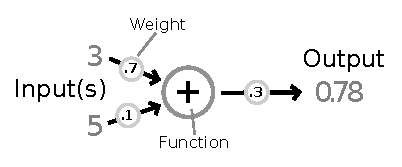
\includegraphics[width=3in]{./pycritters_figs/Neuron.eps}}
\afterfig

In this example of a sum node, the input values {\tt (3,5)} yield 0.78 as the output: 
$(0.7\times 3)+(0.1\times 5) \Rightarrow 2.6$; $2.6 \times 0.3 \Rightarrow 0.78$. 
The function of a given neuron could be any operation on a set of numbers, including 
(but not limited to) difference, product, and sine. More complicated nodes can 
have a memory component.

The simplest type of NN is known as a {\em feed forward} network, which cannot contain cycles and involves {\em hidden} computation layers that act on the values 
of several input nodes and yield values for one or more output nodes:
\index{feed forward neural network}

\beforefig
\centerline{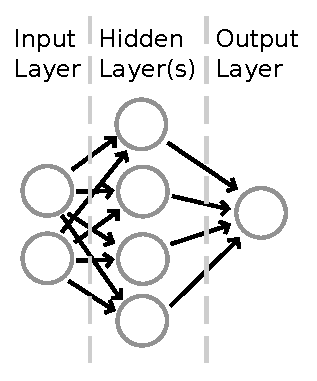
\includegraphics[width=2in]{./pycritters_figs/NN.eps}}
\afterfig

NNs like this can be used effectively for tasks like optical character
recognition (converting handwriting or scanned documents into text). However,
Sims' virtual creatures used more complicted neural networks with no clear
separation between the layers of the network:

\beforefig
\centerline{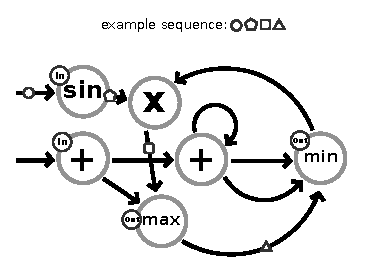
\includegraphics[width=2.5in]{./pycritters_figs/ComplexNN.eps}}
\afterfig

In this example, we follow a sequence of four data elements as they travel 
through the network (obviously, the values change every time they move between 
nodes, but this isn't shown in the diagram). Note that the weights of the edges 
aren't shown and that the second input node's data stream would move in sync 
with the stream that is depicted above. Depending on the implementation of the 
network, edges that have never encountered data before are ignored or assigned a 
value of zero when they propagate data to the nodes.

\section{Body Model}

\section{PyCritters: A Simplified Implementation}

\TODO{Discussion of Results}

\section{The Blind Watchmaker}

As we have seen, complicated systems do not necessarily need to be designed that
way; great complexity (such as that seen in Karl Sim's virtual creatures and in the pycritters) 
can arise from simple processes. This is a counter point to the {\em watchmaker
argument} made famous by the philosopher William Paley in 1802. 
\index{Paley, William}
\index{Watchmaker argument}

The argument follows this basic
framework\footnote{\url{wikipedia.org/wiki/Watchmaker_analogy}}:

\begin{enumerate}
  \item Watches are complex, and if you saw one, you would know that it was made
  by an {\em intelligent designer}, a watchmaker.

  \item {\tt X}, just like a watch, is complex, where {\tt X} is an organ, a
  creature, or anything else. Therefore, it too was created by
  an intelligent designer.
\end{enumerate}

Evolutionary biologist Richard Dawkins refuted this argument in his 1986 book
{\em The Blind Watchmaker: Why the Evidence of Evolution Reveals a Universe
without Design}, in which he used the mammalian eye as an example of a complex
system that could plausibly be the product of natural selection rather than the
result of intelligent design.
\index{Blind Watchmaker@{\em The Blind Watchmaker: Why the Evidence of Evolution Reveals a Universe without Design}}
\index{Dawkins, Richard}

To further prove his point, Dawkins created a computer simulation of {\em
biomorphs}, two dimensional shapes that ``evolved'' based on user selected
mutations.\footnote{\url{wikipedia.org/wiki/The_Blind_Watchmaker}}
\index{Biomorphs}

Karl Sims' virtual creatures can be viewed as a more convincing extension of this early work by
Dawkins, because it doesn't require user interaction to create complex behavior.

\begin{ex}
  Find one of the open source implementations of Dawkins' original Biomorphs
  program, which is called {\em The Blind Watchmaker}, like his book. Can you create 
  seemingly complex shapes with it? If you have time, try to automate the selection process
  by modifying the source code. 
\end{ex}
